\documentclass[10pt, hyperref={bookmarks=false}, show notes]{beamer}
% Text
        \usepackage[T1]{fontenc}
        \usepackage[utf8]{inputenc}
        \usepackage[english]{babel}
        \usepackage[bitstream-charter]{mathdesign} % Serif font (Charter BT).
        \usepackage[scaled=0.84]{DejaVuSansMono} % Monospaced font.
        \def\sfdefault{SourceSansPro-TLF} % Sans serif font.
        \usepackage{textcomp}

% Maths
  \usepackage{amsmath}
  \usepackage{mathtools}
  \usepackage{siunitx}
  % Vector command
  \newcommand{\omatrix}[1]{\ensuremath{\boldsymbol{#1}}}

% Graphics
  \usepackage{graphicx}
  \usepackage[caption=false]{subfig}
        \usepackage{tikz}
  \usepackage{pgfplots}
  \pgfplotsset{compat=1.10}
        % ADD TIKZ LIBRARIES
  \usetikzlibrary{calc}
  \usetikzlibrary{arrows.meta}
  \usepackage{tikz-qtree}
  \usetikzlibrary{decorations.pathmorphing}
  \usetikzlibrary{matrix,shapes,positioning,fit}
  \usepgfplotslibrary{external}
  \tikzexternalize[prefix=graphics/tikz/]
  \tikzexternaldisable % Disable by default
  \usepackage{tabularx}
  \usepackage{pgfgantt}
  \usepackage{multirow}
  \usepackage{hhline}
  
  \usetikzlibrary{positioning,chains,fit,shapes,calc}
  \newcommand\mytext[1][\scriptsize]{#1}

        \usepackage{xcolor}
    \definecolor{color1}{cmyk}{100,50,0,0}   % blue
    \definecolor{color2}{cmyk}{0,80,100,0}   % vermillion
    \definecolor{color3}{cmyk}{97,0,75,0}    % blueish green
    \definecolor{color4}{RGB}{204,121,167}    % reddish purple
    \definecolor{color5}{RGB}{230,159,0}   % orange
   \usepackage{colortbl}
% Misc
\usepackage{booktabs}
\usepackage{enumerate}
\usepackage{pdfpages}
\usepackage{pgfpages}
\usepackage{setspace}
\usepackage{adjustbox}
%\usepackage{multimedia}
\usepackage{changepage}


\setbeamertemplate{navigation symbols}{}
\setbeamertemplate{caption}{\raggedright\insertcaption\par}
%\setbeamertemplate{bibliography item}[text]

\usepackage{caption}
\usetheme{/amsterdam}
\date

\usepackage{beamertheme/handoutWithNotes}
% Uncomment for handouts. Add \documentclass[12pt,handout]{beamer}
%\pgfpagesuselayout{4 on 1 with notes}[a4paper,border shrink=5mm]
% Comment for handouts.
%\setbeameroption{show notes on second screen=right}

% Table of content dybde (0-index)
%\setcounter{tocdepth}{1}

% BibLaTeX
%\usepackage{csquotes}
%\usepackage[
%backend=bibtex,
%citestyle=numeric,
%bibstyle=numeric,
%maxcitenames=3,
%maxbibnames=99,
%url=true]{biblatex}
%\addbibresource{../rapport/references/refs.bib}
%\addbibresource{extrasources.bib}
%\usepackage{../style/biblatex_custom_formatting}

\graphicspath{{graphics/}{../../Report/graphics/}}

\begin{document}

%\captionsetup[figure]{font=small,singlelinecheck=off,justification=raggedright}

\title[Beyond Individual Recommendation]{TrashVision}
\author[\insertframenumber /\inserttotalframenumber]{Lasse D. Christensen, Lukas N. Dalgaard}

\begin{frame}
\Large Beyond Individual Recommendation\\
\normalsize Aggregation Methods for Group Based Recommender Systems \\
\small Lasse D. Christensen, Lukas N. Dalgaard\\
\end{frame}

\begin{frame}
  \frametitle{Contents}
  \tableofcontents
  \note{
  \begin{itemize}
    \item Previous Semester
    \item Current Semester
    \item Evaluation
    \item Contributions
    \item Data Collection 
  \end{itemize}
}
\end{frame}

% PUT INPUTS HERE
\section{Previous Semester}
\begin{frame}
     \begin{center}
     	\huge Previous Semester
     \end{center}
\end{frame}

\begin{frame}
\frametitle{Previous Semester}
\begin{center}
\textit{How can recommendations be made to a group of people by reflecting a groups decision making process, ensuring a high level of satisfaction in the group?}
\end{center}

Working with the assumption that Borda Count was a good mediator but could be improved

\begin{itemize}
\item Borda Transferable Count - Mix of Borda Count and Single Transferable Vote
\item Borda Escalating Count - Having a multiplication factor depending on the item rank
\item Borda Weighted Count - Gets assigned additional points based on the amount if lists an item occurs on
\end{itemize}
\end{frame}

\begin{frame}
\frametitle{Thesis Questions}
\begin{itemize}
\item How does Borda Count perform compared to state-for-the-art rank aggregation methods?
\item How does Borda Count perform on a dataset for group recommendation?
\item How does rearranging top-k lists influence the groups satisfaction?
\end{itemize}
\end{frame}

\section{Current Semester}
\begin{frame}
     \begin{center}
     	\huge Current Semester
     \end{center}
\end{frame}

\begin{frame}
\frametitle{Group Recommendation System}
\begin{columns}
	\begin{column}{0.55\textwidth}
		Individual Recommendations
		\begin{itemize}
			\small
			\item Trained matrix with the predicted individual ratings
			\normalsize
		\end{itemize}
		Groups
		\begin{itemize}
			\small
			\item Artificial constructed groups used for testing
			\normalsize
		\end{itemize}
		Group Recommendation
		\begin{itemize}
			\item Preprocessing 
			\begin{itemize}
				\item Formatting individual lists into ranked top-k lists
			\end{itemize}
			\item Rank aggregation 
			\begin{itemize}
				\item Performing the aggregation and returns the recommendations
			\end{itemize}
		\end{itemize}
		Evaluation
		\begin{itemize}
			\small
			\item An extensive test setup for the evaluation
			\normalsize
		\end{itemize}
	\end{column}
	\begin{column}{0.45\textwidth}
		\begin{figure}
			\centering
			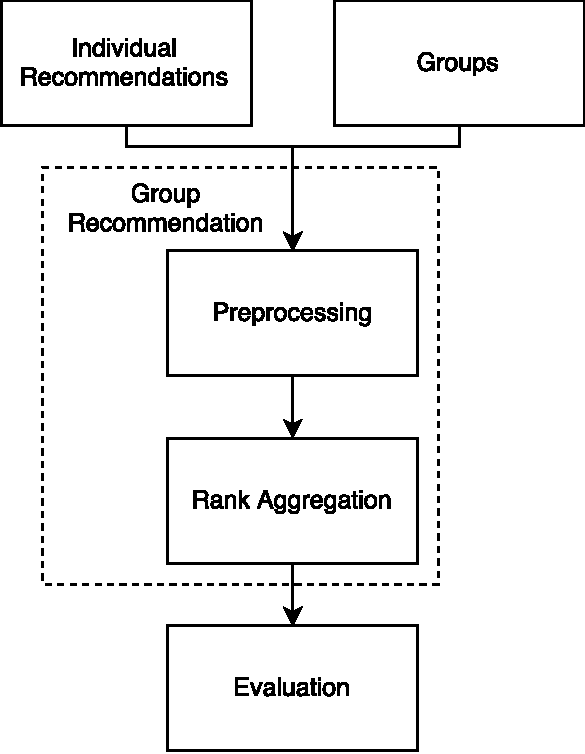
\includegraphics[scale=.5]{graphics/composition}
		\end{figure}
	\end{column}
\end{columns}
\end{frame}

\begin{frame}
\frametitle{Alternative Aggregation Methods}
\begin{columns}
	\begin{column}{0.5\textwidth}
		Voting systems
		\begin{itemize}
			\item Borda Count
		\end{itemize}
		Graph based methods
		\begin{itemize}
			\item Markov Chain 
			\item Spearman's Footrule
		\end{itemize}
		Others
		\begin{itemize}
			\item Average
		\end{itemize}
	\end{column}
	\begin{column}{0.5\textwidth}
		\begin{figure}
			\centering
			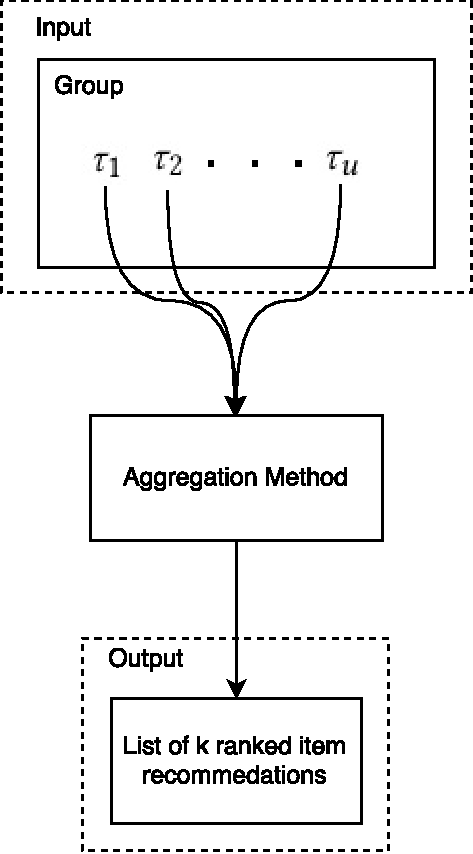
\includegraphics[scale=.4]{graphics/setuptransposed}
		\end{figure}
	\end{column}
\end{columns}
\end{frame}

%\begin{frame}
%\frametitle{Aggregation Methods}
%
%\end{frame}
\section{Results}

\begin{frame}
     \begin{center}
     	\huge Results 
     \end{center}
\end{frame}

\begin{frame}
	\frametitle{Methodology}
	The setup of the new test is the same as the previous tests
	\begin{itemize}
		\item The exact same random generated groups as in the previous tests
		\item Groups of the sizes 4, 8, 12, 16, 20, and 40
		\item There are 1000 groups of each size
		\item The preferences looked at is the top 10
	\end{itemize}
\end{frame}

\begin{frame}
\frametitle{Group Size 4}
\begin{figure}[h]
\centering
\begin{minipage}{.46\textwidth}\centering
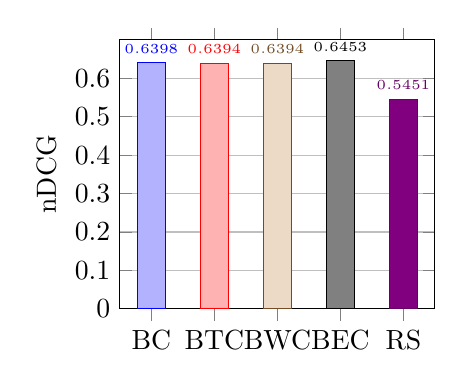
\begin{tikzpicture}
 \begin{axis}[
 	height=5cm,
 	width=4cm,
 	ybar =-10pt,
 	x = .8cm,
 	ymin=0.0, 
 	ymax=0.70,
 	ytick = {0, 0.1,0.2,0.3,...,0.70},
 	scaled y ticks = false,
	enlarge x limits ={abs=.4cm},
	nodes near coords,
    every node near coord/.append style={font=\tiny,/pgf/number format/.cd,precision=4},
 	ylabel={nDCG},
	xtick={0,1,2,3,4},  % NEW BIT
	xticklabels={BC, BTC, BWC, BEC, RS},
	%legend style={at={(0.5,-0.1)},
	%anchor=north,legend columns=-1},
	ymajorgrids = true,]

		\addplot coordinates {(0,0.6398)};    
		\addplot coordinates {(1,0.6394)};    
		\addplot coordinates {(2,0.6394)};    
		\addplot coordinates {(3,0.6453)};    
		\addplot coordinates {(4,0.5451)};
        %\legend{BC, BTC, BWC, BEC, Random}
     \end{axis}
\end{tikzpicture}
\end{minipage}
\begin{minipage}{.46\textwidth}\centering
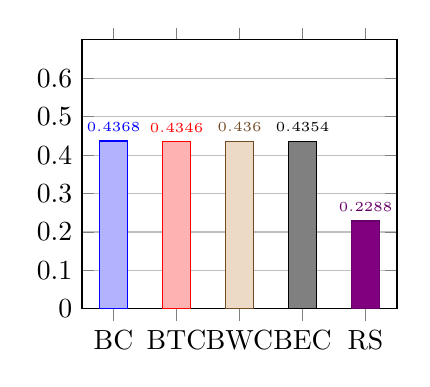
\begin{tikzpicture}
 \begin{axis}[
 	height=5cm,
 	ybar =-10pt,
 	x = .8cm,
 	ymin=0.0, 	
 	ymax=0.70,
 	ytick = {0,0.1,0.20,0.3,...,0.70},
	enlarge x limits ={abs=.4cm},
	nodes near coords,
    every node near coord/.append style={font=\tiny,/pgf/number format/.cd,precision=4},
	xtick={0,1,2,3,4},  % NEW BIT
	xticklabels={BC, BTC, BWC, BEC, RS},
	%legend style={at={(0.5,-0.1)},
	%anchor=north,legend columns=-1},
	ymajorgrids = true,]

		\addplot coordinates {(0,0.4368)};    
		\addplot coordinates {(1,0.4346)};    
		\addplot coordinates {(2,0.436)};    
		\addplot coordinates {(3,0.4354)};    
		\addplot coordinates {(4,0.2288)};
        %\legend{BC, BTC, BWC, BEC, Random}
     \end{axis}
\end{tikzpicture}
\end{minipage}
\end{figure}
\end{frame}

\begin{frame}
\frametitle{Group Size 12}
\begin{figure}[h]
\centering
\begin{minipage}{.46\textwidth}\centering
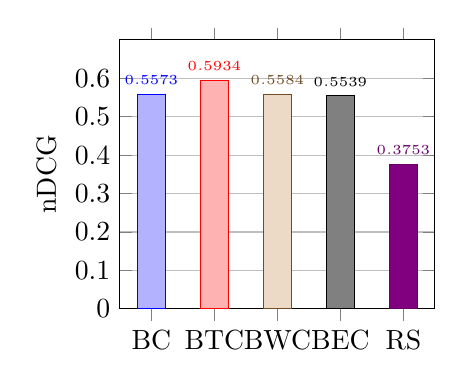
\begin{tikzpicture}
 \begin{axis}[
 	height=5cm,
 	width=4cm,
 	ybar =-10pt,
 	x = .8cm,
 	ymin=0.00, 
 	ymax=0.70,
 	ytick = {0,0.1,0.2,0.3,...,0.70},
 	scaled y ticks = false,
	enlarge x limits ={abs=.4cm},
	nodes near coords,
    every node near coord/.append style={font=\tiny,/pgf/number format/.cd,precision=4},
 	ylabel={nDCG},
	xtick={0,1,2,3,4},  % NEW BIT
	xticklabels={BC, BTC, BWC, BEC, RS},
	%legend style={at={(0.5,-0.1)},
	%anchor=north,legend columns=-1},
	ymajorgrids = true,]

		\addplot coordinates {(0,0.5573)};    
		\addplot coordinates {(1,0.5934)};    
		\addplot coordinates {(2,0.5584)};    
		\addplot coordinates {(3,0.5539)};    
		\addplot coordinates {(4,0.3753)};
        %\legend{BC, BTC, BWC, BEC, Random}
     \end{axis}
\end{tikzpicture}
\end{minipage}
\begin{minipage}{.46\textwidth}\centering
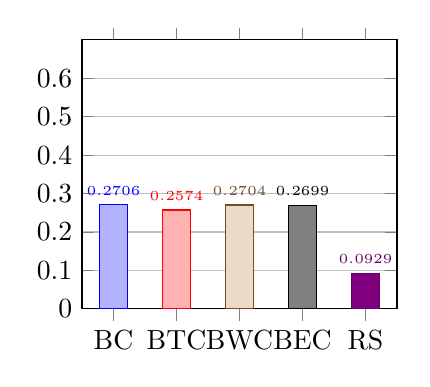
\begin{tikzpicture}
 \begin{axis}[
 	height=5cm,
 	ybar =-10pt,
 	x = .8cm,
 	ymin=0.0, 	
 	ymax=0.70,
 	ytick = {0,0.1,0.20,0.3,...,0.70},
	enlarge x limits ={abs=.4cm},
	nodes near coords,
    every node near coord/.append style={font=\tiny,/pgf/number format/.cd,precision=4},
	xtick={0,1,2,3,4},  % NEW BIT
	xticklabels={BC, BTC, BWC, BEC, RS},
	%legend style={at={(0.5,-0.1)},
	%anchor=north,legend columns=-1},
	ymajorgrids = true,]

		\addplot coordinates {(0,0.2706)};    
		\addplot coordinates {(1,0.2574)};    
		\addplot coordinates {(2,0.2704)};    
		\addplot coordinates {(3,0.2699)};    
		\addplot coordinates {(4,0.0929)};
        %\legend{BC, BTC, BWC, BEC, Random}
     \end{axis}
\end{tikzpicture}
\end{minipage}
\end{figure}
\end{frame}

\begin{frame}
\frametitle{Group Size 40}
\begin{figure}[h]
\centering
\begin{minipage}{.46\textwidth}\centering
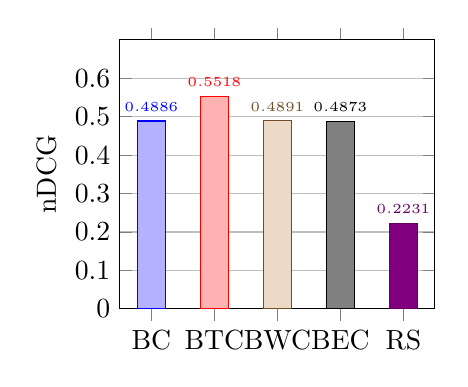
\begin{tikzpicture}
 \begin{axis}[
 	height=5cm,
 	width=4cm,
 	ybar =-10pt,
 	x = .8cm,
 	ymin=0.00, 
 	ymax=0.70,
 	ytick = {0,0.1,0.20,0.3,0.4,0.5,0.60},
 	scaled y ticks = false,
	enlarge x limits ={abs=.4cm},
	nodes near coords,
    every node near coord/.append style={font=\tiny,/pgf/number format/.cd,precision=4},
 	ylabel={nDCG},
	xtick={0,1,2,3,4},  % NEW BIT
	xticklabels={BC, BTC, BWC, BEC, RS},
	%legend style={at={(0.5,-0.1)},
	%anchor=north,legend columns=-1},
	ymajorgrids = true,]

		\addplot coordinates {(0,0.4886)};    
		\addplot coordinates {(1,0.5518)};    
		\addplot coordinates {(2,0.4891)};    
		\addplot coordinates {(3,0.4873)};    
		\addplot coordinates {(4,0.2231)};
        %\legend{BC, BTC, BWC, BEC, Random}
     \end{axis}
\end{tikzpicture}
\end{minipage}
\begin{minipage}{.46\textwidth}\centering
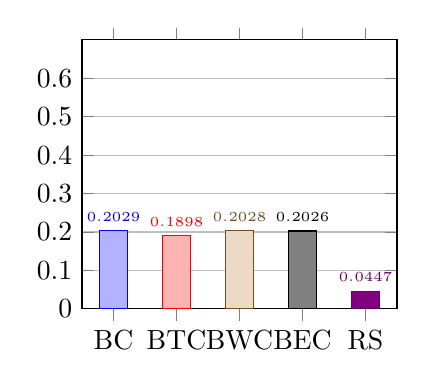
\begin{tikzpicture}
 \begin{axis}[
 	height=5cm,
 	ybar =-10pt,
 	x = .8cm,
 	ymin=0.0, 	
 	ymax=0.70,
 	ytick = {0,0.1,0.20,0.3,0.4,0.5,0.60},
	enlarge x limits ={abs=.4cm},
	nodes near coords,
    every node near coord/.append style={font=\tiny,/pgf/number format/.cd,precision=4},
	xtick={0,1,2,3,4},  % NEW BIT
	xticklabels={BC, BTC, BWC, BEC, RS},
	%legend style={at={(0.5,-0.1)},
	%anchor=north,legend columns=-1},
	ymajorgrids = true,]

		\addplot coordinates {(0,0.2029)};    
		\addplot coordinates {(1,0.1898)};    
		\addplot coordinates {(2,0.2028)};    
		\addplot coordinates {(3,0.2026)};    
		\addplot coordinates {(4,0.0447)};
        %\legend{BC, BTC, BWC, BEC, Random}
     \end{axis}
\end{tikzpicture}
\end{minipage}
\end{figure}
\end{frame}

\begin{frame}
	\frametitle{Possible Solutions}
	\begin{itemize}
		\item Calculate nDCG using the predicted ratings
		\item Ordering the individual ranked list by the average for the group
	\end{itemize}
\end{frame}
\section{Contributions}
\begin{frame}
     \begin{center}
     	\huge Contributions
     \end{center}
\end{frame}

\begin{frame}
\frametitle{Contributions}
Article Contributions
\begin{itemize}
	\item Aggregation methods
	\begin{itemize}
		\item Borda Count
		\item Markov Chain
	\end{itemize}
	\item Baltrunas et al's findings
	\begin{itemize}
		\item Beyond group size 8
	\end{itemize}
\end{itemize}
\hrule \smallskip
Project Findings
\begin{itemize}
	\item Dataset
	\begin{itemize}
		\item Incomplete
		\item Intermediate results
	\end{itemize}
	\item Reordering of Top K
\end{itemize}
\end{frame}
\section{Data Collection}

\begin{frame}
     \begin{center}
     	\huge Dataset
     \end{center}
\end{frame}

\begin{frame}
\frametitle{Dataset}
\begin{itemize}
	\item Short about survey
	\item Short about Amazon
\end{itemize}
\end{frame}

\begin{frame}
\frametitle{Data Collection Status}
\begin{itemize}
	\item Server is online
	\begin{itemize}
		\item pictures of linux/putty/digitalocean/db?
	\end{itemize}
\end{itemize}
\end{frame}

\begin{frame}
\frametitle{Intermediate results}
\begin{itemize}
	\item Our measures
	\begin{itemize}
		\item nDCG
		\item Rating nDCG
		\item Kendall Tau Distance
		\item Spearman's footrule Distance
	\end{itemize}
\end{itemize}
\end{frame}

\begin{frame}
\frametitle{Data}
\begin{itemize}
	\item 219 raw responses
	\begin{itemize}
		\item Remove suspicious responses
		\item Remove incomplete responses
	\end{itemize}
	\item 135 actual responses
	\begin{itemize}
		\item 27 for each group size
		\item group size 4 to 8
	\end{itemize}
\end{itemize}
\end{frame}

\begin{frame}
\frametitle{Intermediate results}
\begin{itemize}
	\item Picture for each measure for our limited data
\end{itemize}
\end{frame}

\begin{frame}
\frametitle{Insights}
\begin{itemize}
	\item Humans do better on nDCG
	\item Humans do a bit worse on Rating nDCG
	\item Humans do a bit worse on KTD
	\item Humans do worse on SFD
\end{itemize}
\end{frame}
%\section{Code Review}

\begin{frame}
     \begin{center}
     	\huge Code Review
     \end{center}
\end{frame}

\begin{frame}
	\frametitle{Problems}
	\begin{itemize}
		\item Error in implementation of the DCG and IDCG algorithm
	\end{itemize}

	\begin{equation}\label{eq:background_dcg}
	\text{(I)DCG}_p = \sum_{i=1}^{p}\frac{\textit{rel}_i}{\log_2(i + 1)}
	\end{equation}	
	
	\begin{itemize}
		\item Misconception of how to find the ideal list for IDCG
	\end{itemize}
	
	\begin{table}[h]
		\centering
		\begin{minipage}{.48\textwidth}\centering
			\begin{tabular}{|l|llll|}
				\hline
						& I1 & I4 & I3  & I2    \\ \hline
				James	& 4  & 3  & 2 	& 1	 	\\ \hline
			\end{tabular}
		\end{minipage}
		\hfill
		\begin{minipage}{.48\textwidth}\centering
			\begin{tabular}{|l|llll|}
				\hline
				Group	& I7 & I2 & I5  & I1    \\ \hline
			\end{tabular}
		\end{minipage}
	\end{table}
	
	\begin{table}[h]
		\begin{tabular}{|l|llll|}
			\hline
			Ideal from report	& I1 & I2 & I5  & I7    \\ \hline
			James score			& 4	 & 1  &	0	& 0		\\
			\hline
		\end{tabular}
	\end{table}
\end{frame}

%We have ratings for all users items, use these to determine satisfaction instead of just top-k.
%Use some average ordering of the top-k.
%\section{Results}

\begin{frame}
     \begin{center}
     	\huge Results 
     \end{center}
\end{frame}

\begin{frame}
	\frametitle{Methodology}
	The setup of the new test is the same as the previous tests
	\begin{itemize}
		\item The exact same random generated groups as in the previous tests
		\item Groups of the sizes 4, 8, 12, 16, 20, and 40
		\item There are 1000 groups of each size
		\item The preferences looked at is the top 10
	\end{itemize}
\end{frame}

\begin{frame}
\frametitle{Group Size 4}
\begin{figure}[h]
\centering
\begin{minipage}{.46\textwidth}\centering
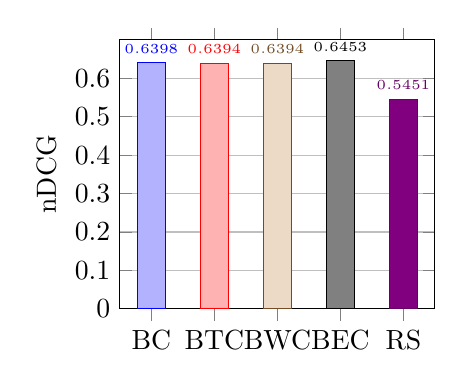
\begin{tikzpicture}
 \begin{axis}[
 	height=5cm,
 	width=4cm,
 	ybar =-10pt,
 	x = .8cm,
 	ymin=0.0, 
 	ymax=0.70,
 	ytick = {0, 0.1,0.2,0.3,...,0.70},
 	scaled y ticks = false,
	enlarge x limits ={abs=.4cm},
	nodes near coords,
    every node near coord/.append style={font=\tiny,/pgf/number format/.cd,precision=4},
 	ylabel={nDCG},
	xtick={0,1,2,3,4},  % NEW BIT
	xticklabels={BC, BTC, BWC, BEC, RS},
	%legend style={at={(0.5,-0.1)},
	%anchor=north,legend columns=-1},
	ymajorgrids = true,]

		\addplot coordinates {(0,0.6398)};    
		\addplot coordinates {(1,0.6394)};    
		\addplot coordinates {(2,0.6394)};    
		\addplot coordinates {(3,0.6453)};    
		\addplot coordinates {(4,0.5451)};
        %\legend{BC, BTC, BWC, BEC, Random}
     \end{axis}
\end{tikzpicture}
\end{minipage}
\begin{minipage}{.46\textwidth}\centering
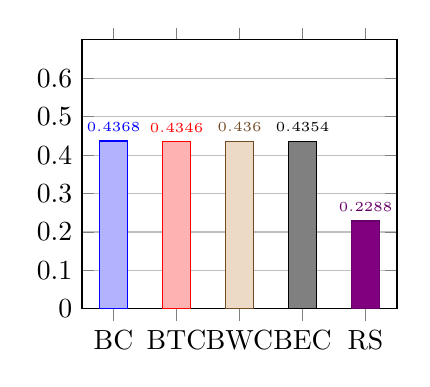
\begin{tikzpicture}
 \begin{axis}[
 	height=5cm,
 	ybar =-10pt,
 	x = .8cm,
 	ymin=0.0, 	
 	ymax=0.70,
 	ytick = {0,0.1,0.20,0.3,...,0.70},
	enlarge x limits ={abs=.4cm},
	nodes near coords,
    every node near coord/.append style={font=\tiny,/pgf/number format/.cd,precision=4},
	xtick={0,1,2,3,4},  % NEW BIT
	xticklabels={BC, BTC, BWC, BEC, RS},
	%legend style={at={(0.5,-0.1)},
	%anchor=north,legend columns=-1},
	ymajorgrids = true,]

		\addplot coordinates {(0,0.4368)};    
		\addplot coordinates {(1,0.4346)};    
		\addplot coordinates {(2,0.436)};    
		\addplot coordinates {(3,0.4354)};    
		\addplot coordinates {(4,0.2288)};
        %\legend{BC, BTC, BWC, BEC, Random}
     \end{axis}
\end{tikzpicture}
\end{minipage}
\end{figure}
\end{frame}

\begin{frame}
\frametitle{Group Size 12}
\begin{figure}[h]
\centering
\begin{minipage}{.46\textwidth}\centering
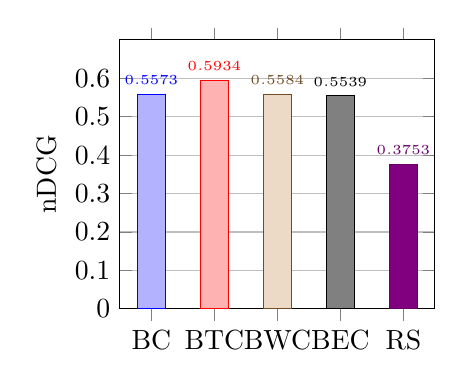
\begin{tikzpicture}
 \begin{axis}[
 	height=5cm,
 	width=4cm,
 	ybar =-10pt,
 	x = .8cm,
 	ymin=0.00, 
 	ymax=0.70,
 	ytick = {0,0.1,0.2,0.3,...,0.70},
 	scaled y ticks = false,
	enlarge x limits ={abs=.4cm},
	nodes near coords,
    every node near coord/.append style={font=\tiny,/pgf/number format/.cd,precision=4},
 	ylabel={nDCG},
	xtick={0,1,2,3,4},  % NEW BIT
	xticklabels={BC, BTC, BWC, BEC, RS},
	%legend style={at={(0.5,-0.1)},
	%anchor=north,legend columns=-1},
	ymajorgrids = true,]

		\addplot coordinates {(0,0.5573)};    
		\addplot coordinates {(1,0.5934)};    
		\addplot coordinates {(2,0.5584)};    
		\addplot coordinates {(3,0.5539)};    
		\addplot coordinates {(4,0.3753)};
        %\legend{BC, BTC, BWC, BEC, Random}
     \end{axis}
\end{tikzpicture}
\end{minipage}
\begin{minipage}{.46\textwidth}\centering
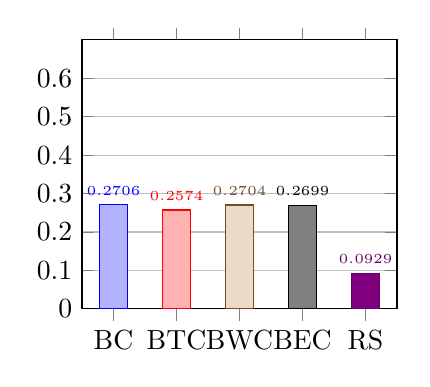
\begin{tikzpicture}
 \begin{axis}[
 	height=5cm,
 	ybar =-10pt,
 	x = .8cm,
 	ymin=0.0, 	
 	ymax=0.70,
 	ytick = {0,0.1,0.20,0.3,...,0.70},
	enlarge x limits ={abs=.4cm},
	nodes near coords,
    every node near coord/.append style={font=\tiny,/pgf/number format/.cd,precision=4},
	xtick={0,1,2,3,4},  % NEW BIT
	xticklabels={BC, BTC, BWC, BEC, RS},
	%legend style={at={(0.5,-0.1)},
	%anchor=north,legend columns=-1},
	ymajorgrids = true,]

		\addplot coordinates {(0,0.2706)};    
		\addplot coordinates {(1,0.2574)};    
		\addplot coordinates {(2,0.2704)};    
		\addplot coordinates {(3,0.2699)};    
		\addplot coordinates {(4,0.0929)};
        %\legend{BC, BTC, BWC, BEC, Random}
     \end{axis}
\end{tikzpicture}
\end{minipage}
\end{figure}
\end{frame}

\begin{frame}
\frametitle{Group Size 40}
\begin{figure}[h]
\centering
\begin{minipage}{.46\textwidth}\centering
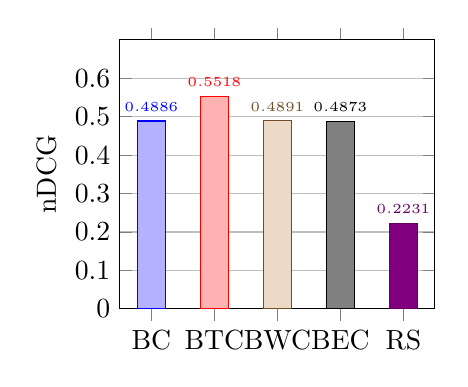
\begin{tikzpicture}
 \begin{axis}[
 	height=5cm,
 	width=4cm,
 	ybar =-10pt,
 	x = .8cm,
 	ymin=0.00, 
 	ymax=0.70,
 	ytick = {0,0.1,0.20,0.3,0.4,0.5,0.60},
 	scaled y ticks = false,
	enlarge x limits ={abs=.4cm},
	nodes near coords,
    every node near coord/.append style={font=\tiny,/pgf/number format/.cd,precision=4},
 	ylabel={nDCG},
	xtick={0,1,2,3,4},  % NEW BIT
	xticklabels={BC, BTC, BWC, BEC, RS},
	%legend style={at={(0.5,-0.1)},
	%anchor=north,legend columns=-1},
	ymajorgrids = true,]

		\addplot coordinates {(0,0.4886)};    
		\addplot coordinates {(1,0.5518)};    
		\addplot coordinates {(2,0.4891)};    
		\addplot coordinates {(3,0.4873)};    
		\addplot coordinates {(4,0.2231)};
        %\legend{BC, BTC, BWC, BEC, Random}
     \end{axis}
\end{tikzpicture}
\end{minipage}
\begin{minipage}{.46\textwidth}\centering
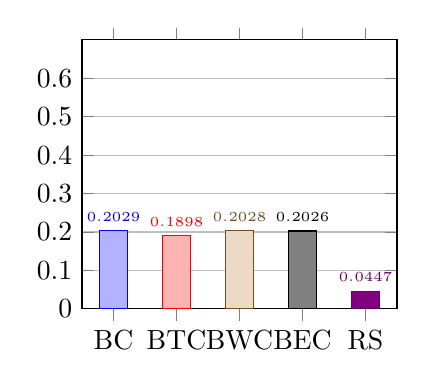
\begin{tikzpicture}
 \begin{axis}[
 	height=5cm,
 	ybar =-10pt,
 	x = .8cm,
 	ymin=0.0, 	
 	ymax=0.70,
 	ytick = {0,0.1,0.20,0.3,0.4,0.5,0.60},
	enlarge x limits ={abs=.4cm},
	nodes near coords,
    every node near coord/.append style={font=\tiny,/pgf/number format/.cd,precision=4},
	xtick={0,1,2,3,4},  % NEW BIT
	xticklabels={BC, BTC, BWC, BEC, RS},
	%legend style={at={(0.5,-0.1)},
	%anchor=north,legend columns=-1},
	ymajorgrids = true,]

		\addplot coordinates {(0,0.2029)};    
		\addplot coordinates {(1,0.1898)};    
		\addplot coordinates {(2,0.2028)};    
		\addplot coordinates {(3,0.2026)};    
		\addplot coordinates {(4,0.0447)};
        %\legend{BC, BTC, BWC, BEC, Random}
     \end{axis}
\end{tikzpicture}
\end{minipage}
\end{figure}
\end{frame}

\begin{frame}
	\frametitle{Possible Solutions}
	\begin{itemize}
		\item Calculate nDCG using the predicted ratings
		\item Ordering the individual ranked list by the average for the group
	\end{itemize}
\end{frame}
%\subsection{Future Work}\label{sec:futurework}
%survey/Dataset 
%Context and influence 
%real world application
%Reordering of rank lists

\begin{frame}
\centering
\huge Questions?
\end{frame}

\begin{frame}
	\begin{center}
		\huge Examples
	\end{center}
\end{frame}

\begin{frame}[t]
\frametitle{Borda Count}
\begin{columns}
\begin{column}{0.5\textwidth}
\begin{align*}
	bc(i) = \sum_{u\in U} \tau_u(i)
\end{align*}
\small
\begin{align*}
	bc(A) = \tau_{u_1}(A) + \tau_{u_2}(A) + \tau_{u_3}(A) + \tau_{u_4}(A)
\end{align*}
\normalsize
\begin{align*}
	bc(A) = 5 + 4 + 2 + 3 = 14
\end{align*}

\end{column}
\begin{column}{0.5\textwidth}
\small
\vspace{-0.5cm}
\begin{table}
\captionsetup{font=footnotesize}
\begin{tabular}{|l|lllll|} \hline
Rank  & 1 & 2 & 3 & 4 & 5 \\\hline
$u_1$ & A & B & C & D & E \\
$u_2$ & C & D & F & A & E \\
$u_3$ & E & A & G & B & D \\
$u_4$ & G & H & A & E & F\\\hline
\end{tabular}
\caption{Top-k list of a group with 4 users}
\end{table}

\vspace{-1cm}
\begin{table}
\begin{tabular}{|l|llllllll|}\hline
      & A & B & C & D & E & F & G & H \\\hline
$u_1$ & 5 & 4 & 3 & 2 & 1 & 0 & 0 & 0 \\
$u_2$ & 2 & 0 & 5 & 4 & 1 & 3 & 0 & 0 \\
$u_3$ & 4 & 2 & 0 & 1 & 5 & 0 & 3 & 0 \\
$u_4$ & 3 & 0 & 0 & 0 & 2 & 1 & 5 & 4 \\\hline
Sum	  & 14& 6 & 8 & 7 & 9 & 4 & 8 & 4 \\\hline
\end{tabular}
\caption{Borda Count scores}
\end{table}
\normalsize
\end{column}
\end{columns}
\begin{table}
\begin{tabular}{llllll}
Recommendations: & A & E & C & G & D
\end{tabular}
\end{table}
\end{frame}

%
%\begin{columns}
%\begin{column}{0.5\textwidth}
%
%\end{column}
%\begin{column}{0.5\textwidth}
%
%\end{column}
%\end{columns}
\subsection{Markov Chain}\label{sec:markovchain}
The proposed Markov Chain method by Dwork et Al, \MC is a generalization of the Copeland Method\note{find cite for this}, where a winner is the candidate which wins the most pairwise contests\citep{rank:aggregation}.

The concept behind building the list of recommendations works by explicitly finding the transition matrix. For \MC, the states are connected to other states that wins per the Copeland method. Then we can iterate through the set, and note who performs best to make the transition matrix. Using the power set on the transition matrix we can find the stationary probability distribution to aggregate the candidates.

The \MC state space corresponds to a set of all the items ranked. The corresponding transition matrix for \MC will have an equal chance of transitioning to any other state that can beat it in a majority of pairwise contests.

Given partial lists $\tau_1,...,\tau_k$, collectively known as $\tau$, with rankings of items, and the state space, $S$, of \MC corresponding to the set of all items ranked in those partial lists. If the current state is item $i$ we can transition to uniformly picked state $j \in S$ where $j$ is ranked higher than item $i$ on a majority of lists in $\tau$ which ranked both $i$ and $j$. Otherwise, we stay in state $i$.

%Non-strict markov chain
\MC as presented by Dwork et al is used on metasearch and aggregating query results, whereas we work in the recommendation domain. To better suit our domain, we make a small adjustment to the method. For search engine comparison, partial lists might not contain both items needed for a pairwise comparison, so in the event of only one item being on the list, it is unknown if the other search engines have ranked the item or not, so Dwork et al restrict themselves to the pairwise comparisons available, and rely on the connectivity in the chain to correct any outcomes.

For our domain we have estimated the rankings giving us a top-k of a full list. So we follow this line of thinking for partial lists containing neither of the items, as the highest rank is not available. However, if the partial list contains one of the items, it wins that pairwise contest, as the losing item is known to be somewhere down the list.

%$p_{ij} = Pr(X_{n+1} = \sum_{l=1}^{k} \tau_l(i) < \tau_l(j) | X_n = \sum_{l=1}^{k} \tau_l(i) > \tau_l(j) )$

%Strict markov chain
%For completeness, we also tested a stricter interpretation of \MC where only the majority winners with both items present were considered.
\begin{frame}[t]
\frametitle{Spearman's Footrule}
\begin{columns}
\begin{column}{0.5\textwidth}
Construct a weighted complete bipartite graph $G(I,P,W)$
\begin{align*}
W(i,p) = \displaystyle\sum_{n=1}^{u} |\frac{\tau_n(i)}{k} - \frac{p}{k}|
\end{align*}

\begin{align*}
W(i,p) = \displaystyle\sum_{n=1}^{u} |\frac{\ell}{k} -\frac{p}{k}|
\end{align*}
\end{column}
\begin{column}{0.5\textwidth}
\definecolor{myblue}{RGB}{80,80,160}
\definecolor{mygreen}{RGB}{80,160,80}
\vspace{-1cm}
\begin{figure}[h]
\begin{tikzpicture}[thick,
  every node/.style={draw,circle},
  fsnode/.style={fill=myblue},
  ssnode/.style={fill=mygreen},
  every fit/.style={ellipse,draw,inner sep=-8pt,text width=2cm},
  ->,shorten >= 2pt,shorten <= 2pt
]

% the vertices of U
\begin{scope}[start chain=going below,node distance=4mm]
\foreach \i in {A,B,C,D,E,F,G,H}
  \node[fsnode,on chain] (f\i) [label=left: \i] {};
\end{scope}

% the vertices of V
\begin{scope}[xshift=3cm,yshift=0cm,start chain=going below,node distance=4mm]
\foreach \i in {1,2,...,8}
  \node[ssnode,on chain] (s\i) [label=right: \i] {};
\end{scope}

% the set U
\node [myblue,fit=(fA) (fH),label=above:$I$] {};
% the set V
\node [mygreen,fit=(s1) (s8),label=above:$P$] {};

% the edges
%\draw[-] (fA) --node[draw=none,fill=none, above]{\mytext[\normalsize]{1}} (s1);
\draw[-] (fA) -- (s1);
\draw[-] (fA) -- (s2);
\draw[-] (fA) -- (s3);
\draw[-] (fA) -- (s4);
\draw[-] (fA) -- (s5);
\draw[-] (fA) -- (s6);
\draw[-] (fA) -- (s7);
\draw[-] (fA) -- (s8);

\draw[-] (fB) -- (s1);
\draw[-] (fB) -- (s2);
\draw[-] (fB) -- (s3);
\draw[-] (fB) -- (s4);
\draw[-] (fB) -- (s5);
\draw[-] (fB) -- (s6);
\draw[-] (fB) -- (s7);
\draw[-] (fB) -- (s8);

\draw[-] (fC) -- (s1);
\draw[-] (fC) -- (s2);
\draw[-] (fC) -- (s3);
\draw[-] (fC) -- (s4);
\draw[-] (fC) -- (s5);
\draw[-] (fC) -- (s6);
\draw[-] (fC) -- (s7);
\draw[-] (fC) -- (s8);

\draw[-] (fD) -- (s1);
\draw[-] (fD) -- (s2);
\draw[-] (fD) -- (s3);
\draw[-] (fD) -- (s4);
\draw[-] (fD) -- (s5);
\draw[-] (fD) -- (s6);
\draw[-] (fD) -- (s7);
\draw[-] (fD) -- (s8);

\draw[-] (fE) -- (s1);
\draw[-] (fE) -- (s2);
\draw[-] (fE) -- (s3);
\draw[-] (fE) -- (s4);
\draw[-] (fE) -- (s5);
\draw[-] (fE) -- (s6);
\draw[-] (fE) -- (s7);
\draw[-] (fE) -- (s8);

\draw[-] (fF) -- (s1);
\draw[-] (fF) -- (s2);
\draw[-] (fF) -- (s3);
\draw[-] (fF) -- (s4);
\draw[-] (fF) -- (s5);
\draw[-] (fF) -- (s6);
\draw[-] (fF) -- (s7);
\draw[-] (fF) -- (s8);

\draw[-] (fG) -- (s1);
\draw[-] (fG) -- (s2);
\draw[-] (fG) -- (s3);
\draw[-] (fG) -- (s4);
\draw[-] (fG) -- (s5);
\draw[-] (fG) -- (s6);
\draw[-] (fG) -- (s7);
\draw[-] (fG) -- (s8);

\draw[-] (fH) -- (s1);
\draw[-] (fH) -- (s2);
\draw[-] (fH) -- (s3);
\draw[-] (fH) -- (s4);
\draw[-] (fH) -- (s5);
\draw[-] (fH) -- (s6);
\draw[-] (fH) -- (s7);
\draw[-] (fH) -- (s8);
\end{tikzpicture}
\caption{Complete bipartite graph}
\end{figure}
\end{column}
\end{columns}
\end{frame}

\begin{frame}[t]
\frametitle{Spearman's Footrule}
\begin{columns}
\begin{column}{0.5\textwidth}
\begin{align*}
W(i,p) = \displaystyle\sum_{n=1}^{u} |\frac{\tau_n(i)}{k} - \frac{p}{k}|
\end{align*}

\begin{align*}
W(i,p) = \displaystyle\sum_{n=1}^{u} |\frac{\ell}{k} - \frac{p}{k}|
\end{align*}
\end{column}
\begin{column}{0.5\textwidth}
\small
\vspace{-0.5cm}
\begin{table}
\captionsetup{font=footnotesize}
\begin{tabular}{|l|lllll|} \hline
Rank  & 1 & 2 & 3 & 4 & 5 \\\hline
$u_1$ & A & B & C & D & E \\
$u_2$ & C & D & F & A & E \\
$u_3$ & E & A & G & B & D \\
$u_4$ & G & H & A & E & F\\\hline
\end{tabular}
\caption{Top-k list of a group with 4 users}
\end{table}
\normalsize
\vspace{1cm}
\end{column}
\end{columns}
\begin{align*}
W(A,1) = (1/5 - 1/5) + (4/5 - 1/5) + (2/5 - 1/5) + (3/5 - 1/5) = 1.2
\end{align*}

\begin{align*}
W(B,1) = (2/5 - 1/5) + (6/5 - 1/5) + (4/5 - 1/5) + (6/5 - 1/5) = 2.8
\end{align*}
\end{frame}

\begin{frame}[t]
\frametitle{Spearman's Footrule}
\begin{columns}
\begin{column}{0.6\textwidth}
\begin{table}[h]
\captionsetup{font=footnotesize}
\footnotesize
\begin{tabular}{|l|llllllll|}\hline
  & 1   & 2   & 3   & 4   & 5   & 6   & 7   & 8   \\\hline
A & 1.2 & 0.8 & 0.8 & 1.2 & 2   & 2.8 & 3.6 & 4.4 \\
B & 2.8 & 2   & 1.6 & 1.2 & 1.2 & 1.2 & 2   & 2.8 \\
C & 2.4 & 2   & 1.6 & 1.6 & 1.6 & 1.6 & 2.4 & 3.2 \\
D & 2.6 & 1.8 & 1.4 & 1   & 1   & 1.4 & 2.2 & 3   \\
E & 2.2 & 1.8 & 1.4 & 1   & 1   & 1.8 & 2.6 & 3.4 \\
F & 3.2 & 2.4 & 1.6 & 1.2 & 0.8 & 0.8 & 1.6 & 2.4 \\
G & 2.4 & 2   & 1.6 & 1.6 & 1.6 & 1.6 & 2.4 & 3.2 \\
H & 3.2 & 2.4 & 2   & 1.6 & 1.2 & 0.8 & 1.6 & 2.4 \\\hline
\end{tabular}
\caption{Calculated weights for the bipartite graph}
\end{table}
\begin{table}
\begin{tabular}{llllll}
Recommendations: & A & G & C & E & D
\end{tabular}
\end{table}
\end{column}
\begin{column}{0.4\textwidth}
\definecolor{myblue}{RGB}{80,80,160}
\definecolor{mygreen}{RGB}{80,160,80}
\vspace{-1.7cm}
\begin{figure}[h]
\begin{tikzpicture}[thick,
every node/.style={draw,circle},
  fsnode/.style={fill=myblue},
  ssnode/.style={fill=mygreen},
  every fit/.style={ellipse,draw,inner sep=-8pt,text width=2cm},
  ->,shorten >= 2pt,shorten <= 2pt
]

% the vertices of U
\begin{scope}[start chain=going below,node distance=3.5mm]
\foreach \i in {A,B,C,D,E,F,G,H}
  \node[fsnode,on chain] (f\i) [label=left: \i] {};
\end{scope}

% the vertices of V
\begin{scope}[xshift=2.5cm,yshift=0cm,start chain=going below,node distance=3.5mm]
\foreach \i in {1,2,...,8}
  \node[ssnode,on chain] (s\i) [label=right: \i] {};
\end{scope}

% the set U
\node [myblue,fit=(fA) (fH),label=above:$I$] {};
% the set V
\node [mygreen,fit=(s1) (s8),label=above:$P$] {};

% the edges
\draw[-] (fA) -- (s1);
\draw[-] (fG) -- (s2);
\draw[-] (fC) -- (s3);
\draw[-] (fE) -- (s4);
\draw[-] (fD) -- (s5);
\draw[-] (fB) -- (s6);
\draw[-] (fF) -- (s7);
\draw[-] (fH) -- (s8);

\end{tikzpicture}
\captionsetup{font=footnotesize}
\caption{Result of minimum cost maximum matching on our bipartite graph}
\end{figure}
\end{column}
\end{columns}
\end{frame}


%\adparagraph{nDCG}

\begin{figure}[H]
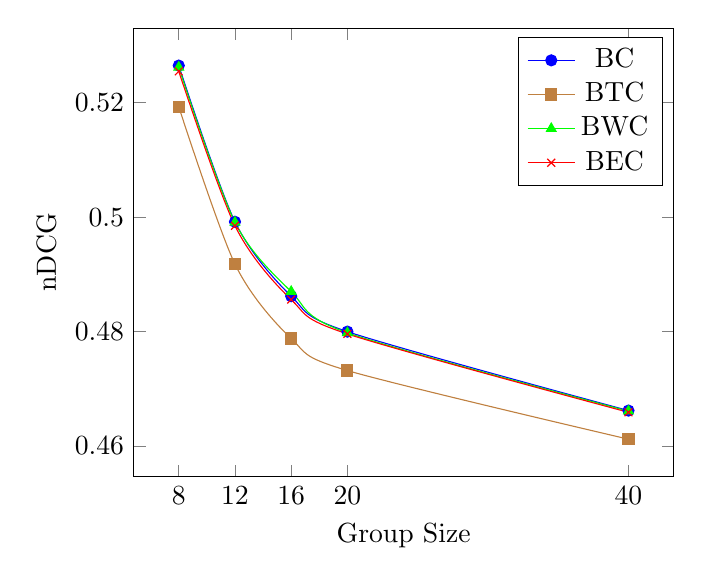
\begin{tikzpicture}
\begin{axis}[
	xlabel=Group Size,
	ylabel=nDCG,
	xtick = {4,8,12,16,20,40}]
		\addplot[smooth,mark=*,blue] plot coordinates {
		%(4,0.6028)
		(8,0.5265)
		(12,0.4992)
		(16,0.4862)
		(20,0.48)
		(40,0.4662)
	};
	\addlegendentry{BC}
	
	\addplot[smooth,color=brown,mark=square*] plot coordinates {
		%(4,0.5995)
		(8,0.5193)
		(12,0.4918)
		(16,0.4788)
		(20,0.4732)
		(40,0.4612)
	};
	\addlegendentry{BTC}
	
	
	\addplot[smooth,color=green,mark=triangle*] plot coordinates {
		%(4,0.6022)
		(8,0.5262)
		(12,0.4991)
		(16,0.487)
		(20,0.4798)
		(40,0.4661)
	};
	\addlegendentry{BWC}
	
	
	\addplot[smooth,color=red,mark=x] plot coordinates {
		%(4,0.6010)
		(8,0.5255)
		(12,0.4985)
		(16,0.4856)
		(20,0.4796)
		(40,0.4659)
	};
	\addlegendentry{BEC}

\end{axis}
\end{tikzpicture}
\caption{Results using nDCG on BC extensions}\label{fig:appendixndcg}
\end{figure}
\begin{frame}[t]
\frametitle{Kendall Tau Distance}
\begin{columns}
\begin{column}{0.5\textwidth}
\footnotesize
\vspace{-0.5cm}
\begin{table}[]
\begin{tabular}{|l|l|l|l|l|}\hline
Par    & $u_4$   & $\omega$ & Case      & Count \\\hline
$G, H$ & $1 < 2$ & $G$      & $case_2$  &       \\
$G, A$ & $1<3$   & $4>1$    & $case_1$  & x     \\
$G,E$  & $1<4$   & $4>2$    & $case_1$  & x     \\
$G,F$  & $1<5$   & $G$      & $case_2$  &       \\
$G,C$  & $G$     & $4>3$    & $case_2$  & x     \\
$G,D$  & $G$     & $4<5$    & $case_2$  &       \\
$H,A$  & $2<3$   & $A$      & $case_2$  & x     \\
$H,E$  & $2<4$   & $E$      & $case_2$  & x     \\
$H,F$  & $2<5$   &          & $case_4$  & x     \\
$H,C$  & $H$     & $C$      & $case_3$  & x     \\
$H,D$  & $H$     & $D$      & $case_3$  & x     \\
$A,E$  & $3<4$   & $1<2$    & $case_1$  &       \\
$A,F$  & $3<5$   & $A$      & $case_2$  &       \\
$A,C$  & $A$     & $1<3$    & $case_2$  &       \\
$A,D$  & $A$     & $1<5$    & $case_2$  &       \\
$E,F$  & $4<5$   & $E$      & $case_2$  &       \\
$E,C$  & $E$     & $2<3$    & $case_2$  &       \\
$E,D$  & $E$     & $2<5$    & $case_2$  &       \\
$F,C$  & $E$     & $C$    	& $case_3$  & x     \\
$F,D$  & $E$     & $D$      & $case_3$  & x     \\
$C,D$  &         & $3<5$    & $case_4$  & x     \\\hline
\end{tabular}
\end{table}
\end{column}
\begin{column}{0.5\textwidth}
\footnotesize
\vspace{-2.5cm}
\begin{table}
\captionsetup{font=footnotesize}
\begin{tabular}{|l|lllll|} \hline
Rank  & 1 & 2 & 3 & 4 & 5 \\\hline
$u_1$ & A & B & C & D & E \\
$u_2$ & C & D & F & A & E \\
$u_3$ & E & A & G & B & D \\
$u_4$ & G & H & A & E & F\\\hline
\end{tabular}
\caption{Top-k list of a group with 4 users}
\end{table}
\normalsize
\begin{itemize}
\item $case_1$: both $i$ and $j$ is in both lists.
\item $case_2$: both $i$ and $j$ is in one list but only one in the other
\item $case_3$: only $i$ or $j$ is in one list and the opposite in the other
\item $case_4$: both $i$ and $j$ is in one list and none in the other
\end{itemize}

\end{column}
\end{columns}
\end{frame}
\subsection*{Spearman's Footrule Distance Example}

\section*{}

\end{document}
